\documentclass{article}
\usepackage[T1]{fontenc}
\usepackage{lmodern}
\usepackage{graphicx}
\usepackage{amsmath,amssymb}
\usepackage[a4paper,margin=2cm]{geometry}
\usepackage[absolute,overlay]{textpos}
\setlength{\TPHorizModule}{1mm}
\setlength{\TPVertModule}{1mm}
\usepackage[indonesian]{babel}
\usepackage{hyperref}
\setlength{\emergencystretch}{2em}
% unit: Halaman 57

\begin{document}

% === Halaman 57 (python/native) ===

57

Kriptografi pada Perang Dunia II

• Perang Dunia ke II, Pemerintah Nazi 

Jerman membuat mesin enkripsi yang 

dinamakan Enigma. 

• Enigma cipher berhasil dipecahkan oleh 

pihak Sekutu.

• Keberhasilan memecahkan Enigma sering 

dikatakan sebagai faktor yang 

memperpendek perang dunia ke-2 

Enigma

% deskripsi: gambar native xref 274
\noindent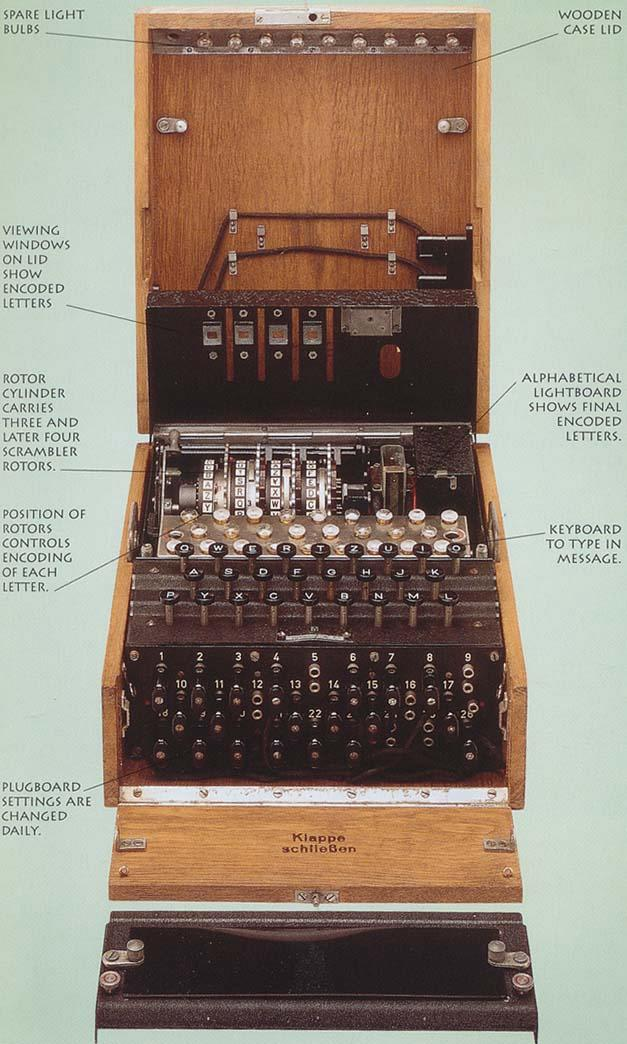
\includegraphics[width=0.85\textwidth]{../../images/python/page_057_img_01.jpeg}

\end{document}
